\subsubsection{\texttt{RF-2}: alta simultánea de ejercicios}
\label{subsec:rf2}

Uno de los procesos más habitualmente repetidos en \textit{VSCode4Teaching} es, desde su primera versión, la subida o adición de nuevos ejercicios dentro de los cursos por parte de los profesores. Este proceso requería necesariamente rellenar un campo de texto con el nombre del ejercicio y seleccionar el fichero, directorio o conjunto de ambos que conformaba la plantilla, subiéndola al servidor y proporcionándosela al alumnado cuando descargasen el ejercicio por primera vez para tomarla como base de su propia propuesta de resolución.

La implementación de este requisito busca crear una nueva forma de subir los ejercicios que simplifique el proceso anteriormente descrito y permita, además, añadir varios ejercicios de una sola vez. En la \referenciaFigura{fig:reqf2-1} se muestra una captura de la extensión en la que se señala el botón para añadir un solo ejercicio (en verde) y el nuevo botón que da acceso a la funcionalidad para subir varios ejercicios en una sola acción (en naranja).

Gracias a la incorporación de esta nueva funcionalidad, los profesores pueden subir varios ejercicios de forma simultánea seleccionando un directorio que tenga en su interior una carpeta para cada ejercicio que se desea crear, de forma que se toma el nombre de cada directorio como el del nuevo ejercicio ---siendo modificable posteriormente---; y sus contenidos, como la plantilla del ejercicio (y la solución, en caso de incluirla, tal como se refleja en la \referenciaSeccion{subsec:rf5}).

\begin{figure}[ht]
    \centering
    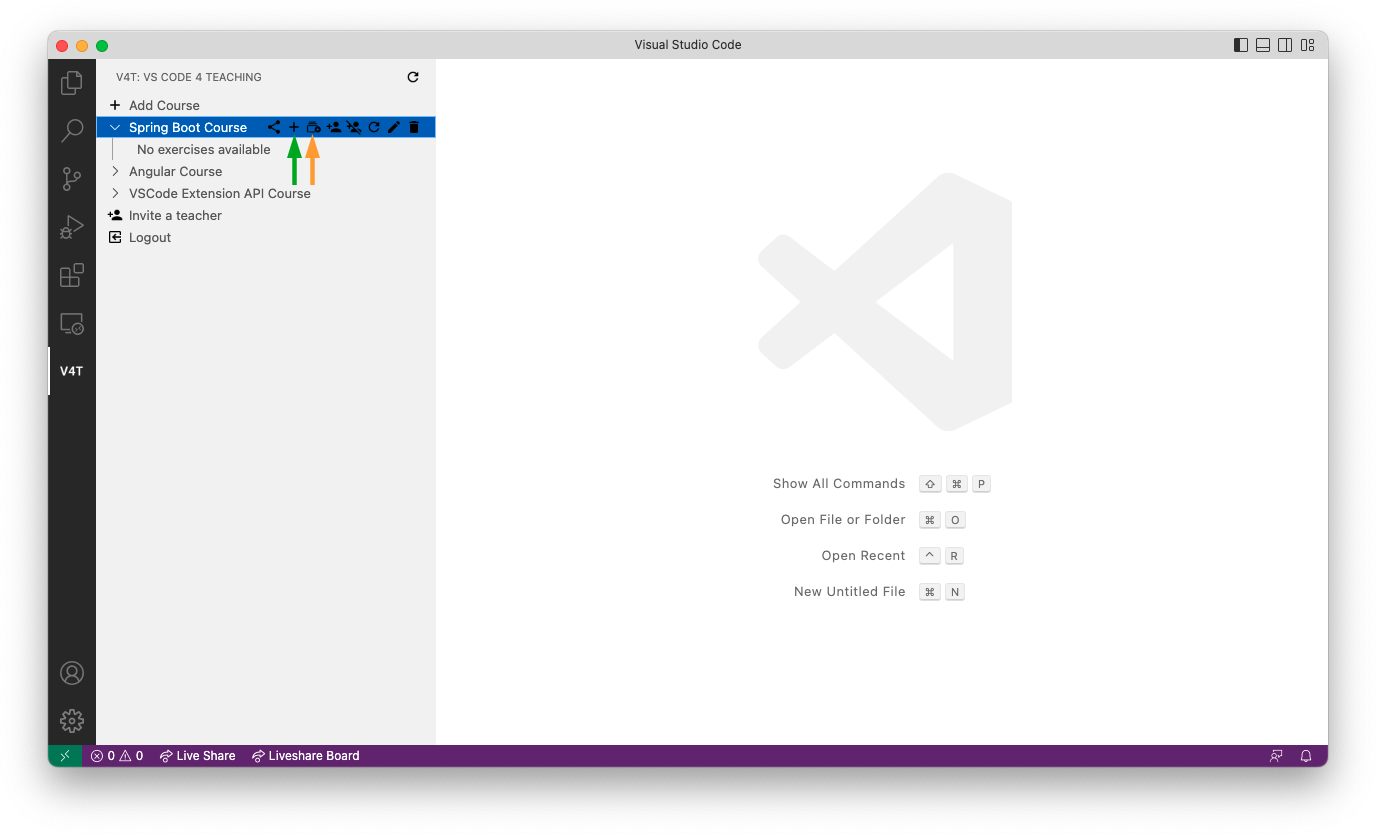
\includegraphics[width=0.975\textwidth]{imagenes/utilizadas/4-3-implementacion/rf2-1.png}
    \caption{Captura de la extensión en la que se destacan los botones empleados para añadir ejercicios.}
    \label{fig:reqf2-1}
\end{figure}
